%% ============================================================================
%% CAPÍTULO 3 - DESARROLLO (Propuesta de desarrollo)
%% ============================================================================

\chapter{PROPUESTA DE DESARROLLO}

En este capítulo se detallan las actividades desarrolladas para cumplir con cada uno de los objetivos específicos planteados, así como las herramientas y técnicas empleadas durante el proceso.

\section{Investigación y puesta en marcha de los motores}

Los servomotores Herkulex DRS-0602, fabricados por Dongbu Robot, son actuadores inteligentes diseñados para aplicaciones en robótica que requieren control preciso de posición, velocidad y torque. Estos motores integran en un mismo módulo el motor DC, el controlador y un sistema de comunicación serial, lo que permite su gestión mediante comandos digitales.

De forma nativa, los servomotores Herkulex se comunican a través de un protocolo UART Multi Drop TTL, descrito por el fabricante como Full Duplex debido a la existencia de líneas diferenciadas de entrada (DIN) y salida (DOUT). Aunque, en configuraciones donde varios actuadores comparten el mismo bus de datos, la comunicación se comporta en la práctica como Half Duplex, ya que únicamente un dispositivo transmite en un instante determinado (Figura~\ref{fig:halffull}).

Para establecer la conexión con una computadora, se utiliza un dispositivo intermedio denominado Herkulex Manager Kit, el cual actúa como interfaz entre el bus de servomotores y el puerto USB de la PC. Esto permite controlar y configurar los motores mediante el software nativo Herkulex Manager, desarrollado por Dongbu Robot. A través de esta interfaz, el software detecta automáticamente los actuadores conectados, posibilitando la realización de tareas de diagnóstico, calibración, asignación de ID y prueba de movimiento.

En este proyecto, debido a la ausencia del Herkulex Hub, se implementó una solución alternativa para establecer la comunicación con los motores. Para ello, se utilizó una placa Arduino Uno modificada, de la cual se retiró el microcontrolador ATmega328P con el fin de aprovechar exclusivamente el módulo de conversión USB--Serial, basado en el chip ATmega16U2. De esta manera, la placa Arduino funcionó como un adaptador USB--TTL, permitiendo la conexión directa entre la PC y el bus de los servomotores, y posibilitando el uso del software Herkulex Manager sin requerir hardware propietario adicional. Esta adaptación permitió la inicialización, reconocimiento y control de los motores Herkulex desde la computadora, reproduciendo parcialmente las funcionalidades del hub original y sirviendo como base para el desarrollo posterior del sistema de control personalizado.

Durante la puesta en marcha se detectaron limitaciones en el software Herkulex Manager, específicamente al intentar modificar los identificadores (ID) de los motores. Si bien el programa permitía realizar la asignación, los valores no se almacenaban de forma persistente, y al reiniciar los servomotores estos retornaban al ID por defecto (256). Para superar esta dificultad, se desarrolló un código en Python que permitió enviar los comandos de configuración directamente a través del puerto serial. Este desarrollo incluyó la creación de una librería propia, dado que las bibliotecas disponibles en línea estaban orientadas a modelos anteriores de la serie Herkulex, tales como los DRS-0101 y DRS-0601, los cuales presentan diferencias significativas en su protocolo de comandos. La nueva librería se diseñó específicamente para el modelo DRS-0602, considerando sus particularidades y limitaciones, y permitió establecer comunicación estable, modificar IDs de forma permanente y ejecutar movimientos básicos mediante comandos personalizados.

En cuanto a la alimentación eléctrica, los servomotores Herkulex DRS-0602 operan dentro de un rango de tensión comprendido entre 9,5\,V y 15\,V, siendo 12\,V el valor óptimo de funcionamiento recomendado por el fabricante. Cada actuador incorpora su propio circuito de control y regulación interna, por lo que resulta fundamental garantizar una fuente de alimentación estable y libre de ruidos, capaz de suministrar la corriente necesaria para el conjunto de motores conectados. Dado que la corriente demandada por cada servomotor puede alcanzar valores del orden de 900\,mA en condiciones de carga máxima, se optó por alimentar los motores mediante una fuente externa dedicada, independiente de la utilizada para la lógica de control. No obstante, se mantuvo una referencia común de tierra (GND) entre la fuente de potencia, la interfaz de comunicación y la computadora, con el fin de asegurar niveles lógicos coherentes en las señales UART TTL.

\begin{figure}[htbp]
  \centering
  
\includegraphics[width=0.7\textwidth]{Esquema_comunicacion.png}
  \caption{Esquema de comunicación. Elaboración propia.}
  \label{fig:comunicacion}
\end{figure}

\begin{figure}[htbp]
  \centering
  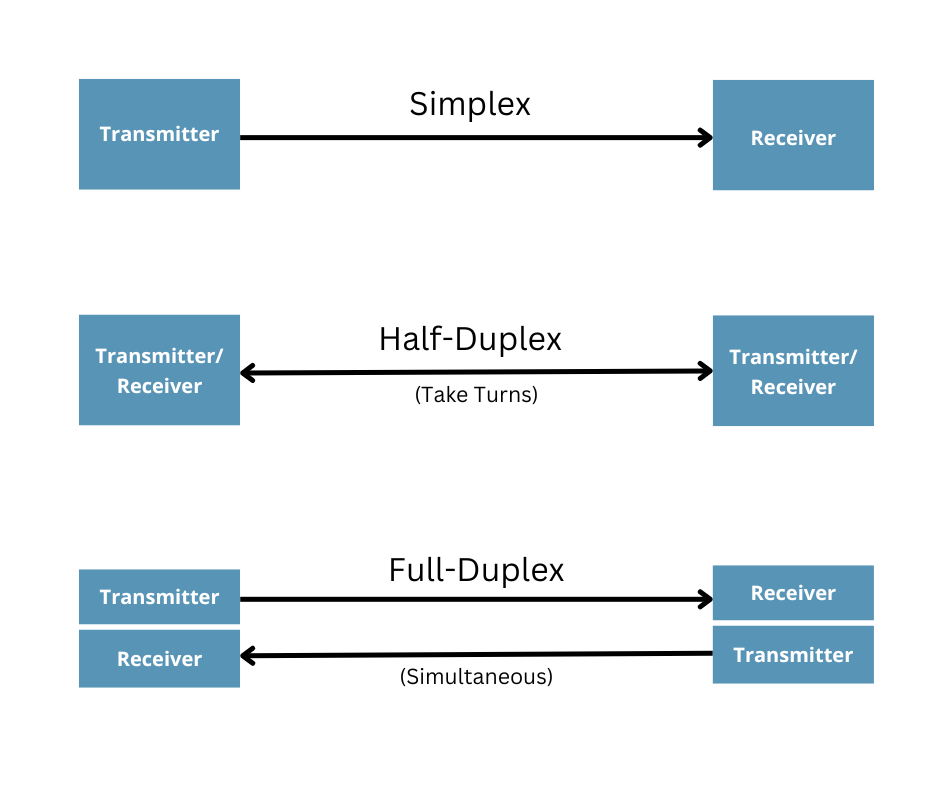
\includegraphics[width=0.6\textwidth]{images/Half-Duplex vs Full-Duplex.png}
  \caption{Half-Duplex vs Full-Duplex. Adaptado de Total Phase.}
  \label{fig:halffull}
\end{figure}

\begin{figure}[htbp]
  \centering
  
\includegraphics[width=0.6\textwidth]{evidencia de proceso.jpg}
  \caption{Diagrama de conexiones y evidencia de proceso. Elaboración propia.}
  \label{fig:conexiones}
\end{figure}

\section{Diseño y desarrollo}

\subsection{Introducción al diseño}

El diseño del cobot tuvo como propósito desarrollar una estructura compacta, modular y mecánicamente estable, capaz de alojar los servomotores Herkulex DRS-0602 respetando su geometría y rango de movimiento. Se buscó una configuración que maximizara el recorrido de cada articulación sin comprometer la rigidez del conjunto, manteniendo proporciones adecuadas para un brazo colaborativo de escritorio y garantizando condiciones seguras de operación.

Dado que el proyecto se enmarca en el desarrollo de un prototipo demostrativo, el enfoque de diseño se centró en lograr una solución simple, accesible y reproducible, capaz de evidenciar los principios básicos de movimiento, control y colaboración entre humano y robot. El diseño no solo buscó satisfacer los requerimientos técnicos del sistema (como el número de grados de libertad, la disposición de los actuadores o la precisión de los movimientos), sino también cumplir con las características esenciales de un robot colaborativo, tales como la seguridad, la suavidad de los bordes, el bajo peso y la limitación de velocidades y esfuerzos.

\subsection{Búsqueda de referencias y análisis de soluciones existentes}

Antes de iniciar el modelado del cobot, se realizó una búsqueda de diseños y desarrollos previos con el objetivo de comprender diferentes enfoques de construcción y soluciones mecánicas aplicadas en brazos robóticos. Se analizaron tanto prototipos académicos y de código abierto disponibles en repositorios en línea (Thingiverse, GrabCAD o CrealityCloud) como robots colaborativos comerciales, entre ellos el KUKA LBR iiwa, el Franka Emika Panda y el Universal Robots UR3.

El análisis de estos modelos permitió identificar distintos métodos de ensamblaje y transmisión de movimiento, así como estrategias de diseño estructural para optimizar la rigidez, el peso y la facilidad de mantenimiento. Si bien los cobots comerciales sirvieron como referencia conceptual en términos de proporciones, geometría y acabados, la implementación mecánica debió ser completamente original, debido a las diferencias en tamaño, componentes y en particular a la utilización de los servomotores Herkulex DRS-0602, para los cuales no existían referencias de integración disponibles.

\subsection{Requerimientos de diseño}

El proceso de diseño del cobot se consolidó a partir de los lineamientos definidos en las etapas previas. Se determinaron los requerimientos técnicos, de seguridad y constructivos que guiaron las decisiones de diseño, fabricación y montaje del sistema. Dado el carácter experimental y demostrativo del proyecto, se optó por fabricar la estructura mediante impresión 3D, priorizando la facilidad de iteración, el bajo costo y la rapidez de producción frente a la resistencia estructural. En esta etapa se seleccionó el material PLA, por su disponibilidad, facilidad de uso y buena estabilidad dimensional.

\begin{table}[htbp]
  \centering
  \caption{Tabla de requerimientos de diseño. Elaboración propia.}
  \label{tab:requerimientos}
  \small
  \begin{tabular}{p{2.2cm}p{3.5cm}p{6.5cm}}
    \toprule
    Categoría & Requerimiento & Descripción \\
    \midrule
    Técnico & Grados de libertad (4 DOF) & Al menos cuatro ejes articulados para movimientos básicos. \\
    & Integración Herkulex DRS-0602 & Montaje preciso, acoples personalizados. \\
    & Comunicación y cableado & Cableado TTL sin interferir con el movimiento. \\
    \midrule
    Seguridad & Movimiento colaborativo & Velocidades y torques limitados. \\
    & Geometría & Superficies redondeadas, sin bordes filosos. \\
    & Zona de trabajo & Alcance máximo adecuado. \\
    \midrule
    Constructivo & Pasaje interno de cables & Canalización para alimentación y señal. \\
    & Modularidad & Módulos reemplazables. \\
    \bottomrule
  \end{tabular}
\end{table}

\subsection{Diseño conceptual y modelado 3D}

El diseño conceptual del cobot se desarrolló a partir del análisis de diferentes modelos de brazos robóticos. El modelado tridimensional se realizó utilizando el software Autodesk Fusion 360, herramienta que permitió definir la geometría de cada componente y evaluar el movimiento relativo entre los ejes. Durante esta etapa se diseñaron las piezas principales que conforman el sistema: la base, los eslabones intermedios, las carcasas de motor y el extremo operativo. Se diseñó de forma modular, donde cada componente puede modificarse o reemplazarse de forma independiente. El resultado final fue un modelo tridimensional de cuatro grados de libertad (4 DOF), diseñado para operar sobre una superficie reducida y servir como plataforma demostrativa para la etapa de programación y control.

\subsection{Impresión 3D y ensamblaje del prototipo}

Construcción del prototipo mediante impresiones 3D, montaje, cableado y ensamblaje. Pruebas iniciales y ajustes realizados para validar el funcionamiento del cobot.
